\documentclass{article}

\usepackage[%
    left=0.5in,%
    right=0.5in,%
    top=0.5in,%
    bottom=0.5in,%
]{geometry}%
\usepackage{minitoc}
\usepackage{multicol}
\usepackage{graphicx}
\usepackage{fixltx2e}
\usepackage{listings}
\usepackage{color}
\usepackage{hyperref}
    \hypersetup{ colorlinks = true, linkcolor = blue }
\usepackage{blindtext}
\definecolor{lightgray}{gray}{0.9}
\graphicspath{ {./} }

\newcommand{\inlinecode}[2]{\colorbox{lightgray}{\lstinline
[language=#1]$#2$}}
\newcommand{\worddef}[1]{\hyperref[sec:reference]{\textit{#1}}}

\begin{document}

\tableofcontents

\newpage

\section{Computer security}
\begin{itemize}
  \item Security is about the protection of assets. Assets might be physical, but they could also be data, information, even ideas
  \item Protection \textbf{measures}: prevention, detection, recovery – manual or automatic
  \item Usually defined as three key areas (CIA):
  \begin{itemize}
    \item \textbf{Confidentiality}: prevention of unauthorised disclosure of information
    \item \textbf{Integrity}: prevention of unauthorised modification of information
    \item \textbf{Availability}: prevention of unauthorised witholding of information or resources
  \end{itemize}
\end{itemize}

\section{Confidentiality}
\begin{itemize}
  \item The prevention of \textbf{unauthorised} users reading private or secret information.
  \item Privacy – The protection of personal data
  \item Examples: medical records, transfer or credit card details
\end{itemize}

\section{Integrity}
\begin{itemize}
  \item The prevention of unauthorised \textbf{modification} of data, and the assurance that data \textbf{remains unmodified}.
  \item Examples: distributed bank transactions, database records
\end{itemize}

\subsection{Integrity vs Authenticity}
\begin{itemize}
  \item Just because we have \textit{integrity}, doesn’t mean we have \textit{authenticity}.
  \item Can we verify the sender? Does it have \worddef{freshness}?
  \item Authenticity is integrity and freshness combined
\end{itemize}

\section{Availability}
\begin{itemize}
  \item The property of being accessible an useable \textbf{upon demand} by an authorised entity
  \item In other words, we want to \textit{prevent denial of service} (DoS)
  \item Examples: redundant power supplies, firewall packet filtering
\end{itemize}

\section{Accountability}
\begin{itemize}
  \item Users should be held responsible for \textbf{their actions} 
  \item The system should \textbf{identify and authenticate} users and ensure compliance 
  \item Audit trails must be kept 
  \item Non-repudiation: a situation where a statement's author cannot \textbf{successfully dispute its authorship} or the validity of an associated contract. Provides un-forgeable evidence that someone did something
\end{itemize}

\section{Data vs information}
\begin{itemize}
  \item Security can be seen as controlling access to information 
  \item This is hard, we usually control access to data instead  
  \begin{itemize}
    \item Data – A means to represent information 
    \item Information – An \textbf{interpretation} of that data 
  \end{itemize}  
  \item Focusing on data can still leave information vulnerable:
  \begin{itemize}
    \item “Mike’s criminal record not found in the database.”
    \item “You do not have permission to access Mike’s criminal record.”
    \item With the second message it can be known that Mike has a criminal record.
  \end{itemize}
\end{itemize}

\section{Security Design principles}

\subsection{Focus of Control}
\begin{flushleft}
In a given application, should the focus of protection mechanisms be
\begin{itemize}
  \item Data: Permitted manipulation of data e.g. consistency check
  \item Operations: Permitted invocations e.g. \verb!transfermoney()!
  \item Users: Permissions for specific users e.g. /home/name/
\end{itemize}
\end{flushleft}

\subsection{Complexity vs. Assurance}
\begin{flushleft}
Would we prefer a simple approach with high assurance, or a feature-rich environment? Feature-rich security systems and high assurance do not match easily. E.g. Linux vs Windows permissions. To achieve a high degree of assurance, the security system has to be examined in close details and exhaustively as possible. Hence, there is a trade-off between complexity and assurance.
\end{flushleft}

\subsection{Decentralised Controls}
\begin{itemize}
  \item Should defining and enforcing security be performed by a central entity, or be left to individual components in a system?
  \item Central Entity – Easy to achieve uniformity, but a possible bottleneck 
  \item Distributed Solution – More efficient, but harder to manage
\end{itemize}

\subsection{Layered Security}
\begin{itemize}
  \item We can visualise our security model in layers 
  \item Each layer protects a boundary, and relies on the security of the layers below
  \item Consider an application using a database:
\end{itemize}
\begin{center}
  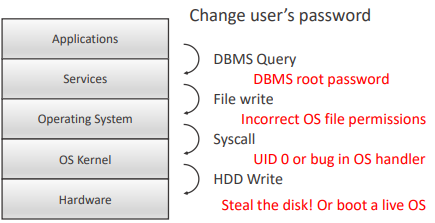
\includegraphics[scale=0.5]{layer_security.png}
\end{center}

\pagebreak
\section*{Reference section} \label{sec:reference}
\begin{description}
	\item[freshness] \hfill \\ Implies that the sensed data are recent, and it ensures that no adversary replayed old messages
\end{description}
\end{document}
